\chapter{Neural Networks}
\section{Introduction to Neural Networks}

In the field of computational research, the use of computers is generally restricted to discreet, exact commands that are meant to be executed in a certain manner, which  provide the computational power required for complex calculations.
In contrast, neural networks are an example of machine learning (ML), wherein the machine is capable of learning behavior or interpreting patterns from a given data set.
The field of predictive analysis uses this paradigm of computational interpretation.
For example, it is extremely challenging to develop a system that is purely programmed to recognize handwriting.
Yet, computers at the United States Postal Service are able to decipher human words and reroute letters and packages without the need for humans.
These computers contain a neural network that has been trained to recognize handwriting and predict characters as they appear on mail. \cite{nielsen} 

\begin{figure}[htbp!]
   \centering
   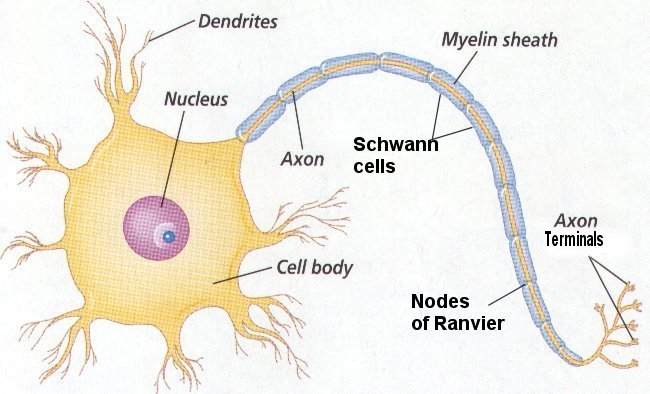
\includegraphics[width=0.5\textwidth]{pictures/NeuralNetworks/neuron.jpg} 
   \caption{The Parts of an Anatomical Neuron}
   \label{fig:neuron}
\end{figure}

Neural networks were designed using the human brain as an inspiration.
The neural network is composed of perceptrons, which are similar to the smallest functional units of the brain: the neuron.
Neurons act as the wiring of the brain by passing along signals that they receive to other neurons.
When a neuron communicates with another neuron, it uses neurotransmitters to either increase or decrease the probability of the next neuron firing.
Thus, a neuron can be excitatory (increases the chance of the next neuron firing) or inhibitory (decreases the chance of the next neuron firing).
Similarly, neural networks utilize perceptrons that can receive multiple inputs and produce a single output.
The inputs are binary values ($0$ or $1$), and affect the perceptron differently depending on their excitatory or inhibitory ability.
The amount of excitation or inhibition is captured by weights, or values that the inputs are multiplied by.
Finally, the aggregate sum of these inputs and their weights is used to calculate if the perceptron in question will fire an output to the next layer of perceptrons. 

\begin{figure}[htbp!]
    \centering
    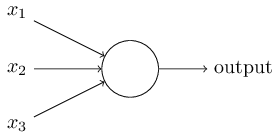
\includegraphics[scale=1.0]{pictures/NeuralNetworks/sigmoidNeuron.png}
        \caption{A neuron in a neural network, with binary inputs $x_1$, $x_2$, and $x_3$.}
    \label{fig:sigmoidNeuron}
\end{figure}

Neurons that only utilize binary inputs, however, are not efficient in learning.
For example, neurons in the brain release different amount of neurotransmitters to indicate different levels of excitation.
Similarly, most modern neural networks generate an output that is between $0$ and $1$, inclusive.
This type of function is known as the sigmoid function, and the resulting neuron is known as the sigmoid neuron. 

\subsection{Neural Networks with Sigmoid Neurons}

With practice, humans can arrange sigmoid neurons to generate a functional unit that can take inputs and produce a certain computational output.
Functionally, sigmoid neurons act as \texttt{NAND} gates, which are universal to computational procedures.
However, the true value of the neural network lies in data and input values that do not have any discernible pattern.
In such cases, neural networks are capable of learning patterns by themselves.
Therefore, neural networks can be trained with an initial data set, after which they can predict the output values of new information.
Although a single sigmoid neurons can be trained, it is not adequate to use such a unit to capture the entirety of complex patterns found in data sets.
Rather, a network of sigmoid neurons is created to assess input values and generate proper outputs.
Neural networks are most often arranged in layers.
The first layer is known as the input layer, whilst the last layer is known as the output layer.
All the neural layers in the middle are known as hidden layers. 
\begin{figure}[htbp!]
    \centering
    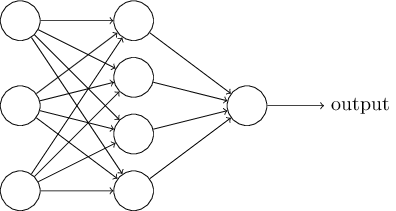
\includegraphics[scale=0.75]{pictures/NeuralNetworks/neuralNetwork.png}
        \caption{A neural network with three layers: an input layer, a hidden layer, and an output layer.}
    \label{fig:neuralNetwork}
\end{figure}
The sample neural network shown in figure \ref{fig:neuralNetwork} takes four inputs in the first layer and produces a singular output.
Since all the components involved are sigmoid neurons, the value of the output of the neural network can take any value between 0 and 1. 

\subsection{Training in a Neural Network}

In general, every sigmoid neuron has a certain set of inputs $X=\{x_1, x_2, \hdots , x_n\}$.
Each input is associated with a weight, or the amount of excitation or inhibition each input causes, which are expressed as the weight set $W=\{w_1, w_2, \hdots , w_n\}$.
The value of the previous inputs is also influenced by a neuron-specific bias $b$, which acts as a value of how reactive the neuron is to the inputs.
Finally, the sigmoid neuron produces an output $O$ between $0$ and $1$ depending on the influence of previous inputs as follows:

\begin{gather*}
    \sigma (x)=\frac{1}{1+e^{-x}}\\
    O(W, X)=\sigma \left(\sum_{i}^{n} w_{i}x_{i} + b\right)\\
    O(W, X)=\sigma \left(W\cdot X + b\right)\\
    O(W, X)=\frac{1}{1+e^{-W\cdot X - b}}
\end{gather*}

Therefore, by computing the dot product of set $W$ and set $X$, offsetting the dot product by the neural bias, and then passing that value through the sigmoid function, we generate an output between 0 and 1.
If the sigmoid neuron in question is part of a hidden layer, it will pass on its output to other neurons in the next lay. 

To train a network, we begin with a neural network that is set up with well-chosen (but random) weights and begin sending input values through it.
The output is then compared to the value we were expecting, and computational corrections are made in increments to the weights and biases in the neural network using gradient descent algorithms.
Over time, the neural network becomes more accurate and has the ability to predict future output values from input values.

\subsection{Measuring Predictive Error}

To train our neural network computationally, we need to develop a cost function, that quantifies the amount of training our neural network has undergone.
That is, this function has to return a value that quanitifies the difference between prediction and reality.
During training, every predicted value is compared to the actual value of the data through subtraction and squared.
Thus, for a prediction $y$ and actual value $\hat y$.

\[
C(y,\hat y)=(\hat y - y)^2
\]

The cost function is computed for every data point used to train the neural network.
The overall error of the neural network is simply the average of all the cost function values for every data point that was used to train the network.
However, since we are squaring the cost function, we divide the average by 2 to decrease the severity of predictive error.
This error function is most commonly known as the Mean-Squared Error function, and is predominantly used to train neural networks.
For a set of predictions $Y=\{y_1,y_2,\hdots,y_n\}$ and a set of actual values $\hat Y=\{\hat y_1,\hat y_2,\hdots,\hat y_n\}$:

\begin{gather*}
J(Y,\hat Y)=\sum_{i=0}^{n} \frac{C(y_i,\hat y_i)}{2n} \\
J(Y,\hat Y)=\sum_{i=0}^{n} \frac{(\hat y_i - y_i)^2}{2n}
\end{gather*}

\section{Installation}

The neuralnet package can be found at \url{https://cran.r-project.org/web/packages/neuralnet/index.html}.
Download the package that works for your operating system and CPU architecture.
The following code can be used to install the package from the R command line.
This example illustrates the installation of a windows system binary file.
However, all other installations will also be the same, with \texttt{FILE\_PATH} leading to the package downloads.
Alternatively, a script file can be generated to install the neuralnet package. 
\begin{figure}[htbp!]
\caption{Code for Windows}
\begin{lstlisting}
install.packages("FILE_PATH.zip", repos=NULL)
package 'neuralnet' successfully unpacked with MD5 sums checked
library(neuralnet)
\end{lstlisting}
\end{figure}

\begin{figure}[htbp!]
\caption{Code for Mac / OSX}
\begin{lstlisting}
install.packages("FILE_PATH.tgz")
package 'neuralnet' successfully unpacked with MD5 sums checked
library(neuralnet)
\end{lstlisting}
\end{figure}

Note that safari automatically decompresses \texttt{.tgz} files to tar files, and this will cause errors when running the above code.
The installation may throw a warning reminding the user that the package may be out-of-date when compared to the R version being used. 

\section{Objectives of Case Study}

There are multiple objectives that the student must accomplish over the course of this neural networks case study.
\begin{enumerate}
\item Understand neural networks, their functional units, and their overall purpose in Machine Learning.
It is important to understand how neural networks work, beginning from an understanding of sigmoid neurons and culminating in an overall appreciation for the function of neural networks in predictive analysis.
\item Have the ability to prepare data for use in neural networks in R.
This objective includes the ability to identify and remove rows with empty data, normalizing the data to allow for learning over a smaller number of iterations, and fitting data curves to create the predictive function.
\item Be able to implement the neuralnet package in R.
An understanding of the functionality that the neuralnet package provides, including creating the neural network, training it with a data set, and using it for predictive analysis, is imperative to this objective.
\item Perform cross-validation on the neural network to confirm understand its learning progress.
This involves using statistical measures to see how the neural network is functioning during training and prediction.
\end{enumerate}
\section{Case Study - Boston Housing Database}

The Boston Housing Database is a databaase that contains the housing data from the boston area.
It contains data on housing sales, including the area of the house sold, the location of the house, and other price-determining factors.

\subsection{Loading and Separating the Data}

Create a R script file and enter the following code.
This code will set up the environment for the neural network.
We load the data into our scripting environment, modify it to fit the neuralnet package, and split it into a training and testing dataset. 
\begin{lstlisting}
# Name:     neural.R
# Author:   First Last
# Date:     Month Date Year

# Load necessary libraries into R
library(neuralnet) # Contains the neuralnet package
library(MASS)      # Contains the database we will use

# Clear the current environmental variables
rm(list=ls())

# We set the seed for the random generator
# We use random data values for training and for testing
# Use this seed to replicate the results in this chapter
set.seed(500)

# Import the database into R from the MASS library
data <- Boston

# Define the number of neurons in each hidden layer
# The input layer depends on the number of columns in the data frame
# The output layer depends on variables we ask the network to predict
hiddenLayers = c(5, 3)
\end{lstlisting}

Unfortunately, the neuralnet package cannot handle \texttt{NULL} values in the data.
Therefore, we must remove such extraneous data from the dataset.

\begin{lstlisting}
# Unlike most R libraries, neuralnet is unable to parse NA values
# We check for NA values in the data set and print their amount
# If we have rows with missing data, we will have to remove them
apply(data, 2, function(x) sum(is.na(x)))
\end{lstlisting}

We will use 75\% of the data to train the network and 25\% to test the efficacy of the neural network.
We split the dataset using the following code.

\begin{lstlisting}
# Generate a list of indices that are randomly sampled
# The indices point to rows in the data
# 75 percent of the data set indices is selected in this list
index <- sample(1:nrow(data), round(0.75 * nrow(data)))

# The training data set is composed of 75 percent of the test data
train <- data[index,]

# The testing data set is composed of 25 percent of the test data
test <- data[-index,]
\end{lstlisting}

\subsection{Linear Model for Comparison}

First, we run the data through a simple linear model to see how well a linearly scaled system can predict the value of interest in the data set.
Our data frame is constructed so that the last column, named \texttt{data\$medv}, is what is predicted.
Every other column is the value of a pixel in the image.

\begin{lstlisting}
# Create a regression line using prog as the prognostic variable
lm.fit <- glm(medv~., data=train)
# Print the summary of our fit
summary(lm.fit)
# Predict values using the fit and the testing data set
lm.pr <- predict(lm.fit, test)
# Calculate the Mean-Square Error of the linear model
lm.MSE <- sum((lm.pr - test$medv)^2) / nrow(test)
\end{lstlisting}

\subsection{Neural Network Setup and Execution}

We will compare the linear model to the neural network graphically after generating results from the neural network.
We now work to set up the data for the neural network.
Neural networks generally do not work well with non-uniform distributions of data.
Therefore, we will scale every column to distribute the values correctly.
When we scale the data set, we will lose the true values.
Therefore, it is important to ``unscale'' the data once we generate output from the network.

\begin{lstlisting}
# Create a list of maximums from each data column
maxs <- apply(data, 2, max)
# Create a list of minimums from each data column
mins <- apply(data, 2, min)

# Scale the values in each column to its respective limits
scaled <- as.data.frame(scale(data, center=mins, scale=maxs - mins))

# Redefine a training data set using the scaled values
train_ <- scaled[index,]
# Redefine a testing data set using the scaled values
test_ <- scaled[-index,]
\end{lstlisting}

At this point, we can generate a neural network and execute it.
We begin by constructing a rule for the neural network to follow.
This rule simply describes the output variables and the input variables that are thought to influence the output. 

\begin{lstlisting}
# Every column affects the prognostic variable
# We extract the name of every column in the data set
n <- names(train_)

# Using the normal fit construct (prog ~) does not work in this package
# Instead, we generate the command using the following code
# Will generate something like this: prog ~ c1 + c2 + c3 + ...
f <- as.formula(paste("medv ~", paste(n[!n %in% "medv"], collapse=" + ")))

# The following code will generate the neural network
# This step can take some time
nn <- neuralnet(f, data=train_, hidden=hiddenLayers, linear.output=T)

# We can plot the neural network to view its structure
plot(nn)
\end{lstlisting}

Just like the linear model that we use to compare, we will calculate the Mean-Squared Error of the neural network.
For this, we extract the predictions of the neural network and ``unscale'' them. 

\begin{lstlisting}
# Compute predictions from our neural network
nn.pr_ <- compute(nn, test_[,1:13])

# Unscale the data output from the neural network
nn.pr <- nn.pr_$net.result * (max(data$medv) - min(data$medv)) + min(data$medv)
test.r <- (test_$medv) * (max(data$medv) - min(data$medv)) + min(data$medv)

# Root Mean Square Error computation for the neural network
nn.MSE <- sum((test.r - nn.pr)^2) / nrow(test_)
\end{lstlisting}

\subsection{Graphical Representation}

Now, we simply use descriptive and graphical methods to highlight the difference between a linear fit model and the neural network.

\begin{lstlisting}
# A higher number will suggest a lower correlation between the prediction and reality
print(paste(lm.MSE, nn.MSE))

# Set up a plot to hold two graphs
par(mfrow=c(1, 2))

# Plot the neural network's real vs. predicted values
plot(test$medv, nn.pr, col="red", main="Real vs. Predicted NN", pch=18, cex=0.7, xlab="Actual Value", ylab="Neural Network")
# Generate a line and legend for the plot
abline(0, 1, lwd=2)
legend("bottomright", legend="LM", pch=18, col="red", bty="n", cex=0.95)

# Plot the linear model's real vs. predicted values
plot(test$prog, lm.pr, col="blue", main="Real vs. Predicted LM", pch=18, cex=0.7, xlab="Actual Value", ylab="Linear Fit")
# Generate a line and legend for the plot
abline(0, 1, lwd=2)
legend("bottomright", legend="LM", pch=18, col="blue", bty="n", cex=0.95)

# Generate a plot with both scatter plots for better comparison
par(mfrow=c(1, 1))
plot(test$medv, nn.pr, col="red", main="Real vs. Predicted", pch=18, cex=0.7, xlab="Actual Value", ylab="Predicted Value")
points(test$medv, lm.pr, col="blue", pch=18, cex=0.7)
abline(0, 1, lwd=2)
legend("bottomright", legend=c("NN", "LM"), pch=18, col=c("red", "blue"))
\end{lstlisting}

A proper execution of the neural network should show that the Mean-Squared Error of the generalized linear fit model is much higher than that of the neural network.
Furthermore, the graphs should portray a tighter clustering of the neural network data points around the linear fit. 

\section{Student Assignment - Temperature Dataset} 

The student is tasked with creating a neural network that interprets a dataset that contains the monthly temperatures from January to November over multiple years.
The goal of the network is to predict the temperatures of the month of December.
The following code should be used to parse the data:

\begin{lstlisting}
# Name:         neuralStudent.R
# Author:       First Last
# Date:         Month Date Year

### PARSING ###

monthlyavg <- c(-4.07, -1.75, 2.17, 8.06, 13.90, 18.77, 21.50, 20.50, 16.27, 9.74, 2.79, -2.36)
rawdata <- read.csv("berkeleyusdata.txt", header = FALSE)
tempdevs <- rawdata$V4
temps <- rawdata$V4 + monthlyavg
months <- rawdata$V3
mat <- matrix(temps,ncol=12)
datafornnet <- data.frame(mat)
colnames(datafornnet) <- c("Jan","Feb","Mar","Apr","May","Jun","Jul","Aug","Sep","Oct","Nov","Prog")
data <- datafornnet
rm(monthlyavg, rawdata, tempdevs, temps, months, mat, datafornnet)
\end{lstlisting}

Thus, the data set is stored in a variable called \texttt{data}.
The neural network can now be built by the students.
The name of the variable being predicted is \texttt{Prog}. 

\begin{lstlisting}
# Clear environment variables
rm(list = ls())

# Import the appropriate libraries
library(neuralnet)

# We do not need to set a seed
# We can if the pseudo-random system creates better results
# set.seed(500)

# Vary the number of neurons in the hidden layers to get better results
# This is an example a student may use
hiddenLayers = c(5, 3)

# Ensure that the data has no NaN values
apply(data, 2, function(x) sum(is.na(x)))

# Split the data into 75% and 25%
# One dataset is for training and the other is for testing
index <- sample(1:nrow(data), round(0.75 * nrow(data)))
train <- data[index,]
test <- data[-index,]

# Create a generalized linear fit to compare with the neural network
lm.fit <- glm(Prog~., data=train)
# Print the summary of the fit
summary(lm.fit)
# Predict values using the fit
lm.pr <- predict(lm.fit, test)
# Calculate the Mean-Squared Error of the model
lm.MSE <- sum((lm.pr - test$Prog)^2) / nrow(test)

# Calculate mins and maxes for scaling
maxs <- apply(data, 2, max)
mins <- apply(data, 2, min)
# Scale using the range of the data
scaled <- as.data.frame(scale(data, center=mins, scale=maxs-mins))
# Create the scaled training and test data sets
train_ <- scaled[index,]
test_ <- scaled[-index,]

# Create the neural network
n <- names(train_)
f <- as.formula(paste("Prog ~", paste(n[!n %in% "Prog"], collapse=" + ")))
nn <- neuralnet(f, data=train_, hidden=hiddenLayers, liner.output=T)
plot(nn)

# Calculate the scaled predictions and errors
nn.pr_ <- compute(nn, test_[,1:11])
nn.pr <- nn.pr_$net.result * (max(data$Prog) - min(data$Prog)) + min(data$Prog)
test.r <- (test_$Prog) * (max(data$Prog) - min(data$Prog)) + min(data$Prog)
nn.MSE <- sum((test.r - nn.pr)^2) / nrow(test_)

# Print the resulting mean-squared errors
print(paste(lm.MSE, nn.MSE))

# Generate the graphics for displaying data
par(mfrow=c(1,2))
plot(test$Prog, nn.pr, col="red", main="Real vs. Predicted NN", pch=18, cex=0.7, xlab="Actual Value", ylab="Neural Network")
abline(0, 1, lwd=2)
legend("bottomright", legend="LM", pch=18, col="red", bty="n", cex=0.95)
plot(test$Prog, lm.pr, col="blue", main="Real vs. Predicted LM", pch=18, cex=0.7, xlab="Actual Value", ylab="Linear Fit")
abline(0, 1, lwd=2)
legend("bottomright", legend="LM", pch=18, col="blue", bty="n", cex=0.95)
par(mfrow=c(1,1))
plot(test$Prog, nn.pr, col="red", main="Real vs. Predicted", pch=18, cex=0.7, xlab="Actual Value", ylab="Predicted Value")
points(test$Prog, lm.pr, col="blue", pch=18, cex=0.7)
abline(0, 1, lwd=2)
legend("bottomright", legend=c("NN", "LM"), pch=18, col=c("red", "blue"))
\end{lstlisting}

\section{Downloading The Dataset}

The data can be found in the github folder associated with this chapter of the textbook.
This data comes from the Berkeley Earth Project.
